
\begin{frame}{¿C\'omo?}
    \begin{block}<2>{}
        La forma m\'as sencilla de almacenar datos es escribirlos en un fichero
    \end{block}
    \vspace{5mm}

    \centering
    \includegraphics<2>[width=50mm, height=50mm]{img/csv.png}
\end{frame}


\begin{frame}{Sistemas orientados a ficheros}
   
    \begin{columns}[T]
        \begin{column}{0.30\linewidth}
            \begin{block}
                
                \begin{tabular}{c c c}
    
                    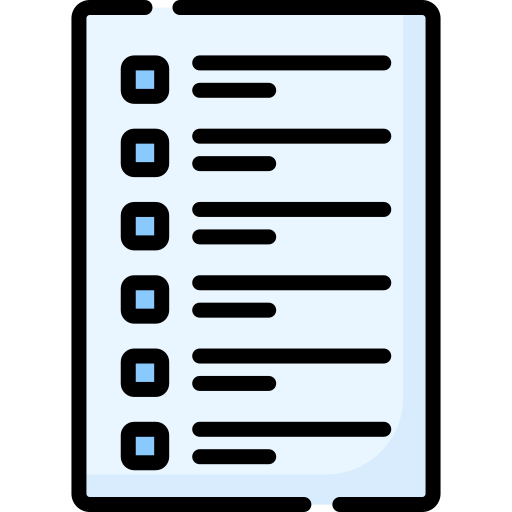
\includegraphics[width=1cm]{img/list.png}
                    
                    & 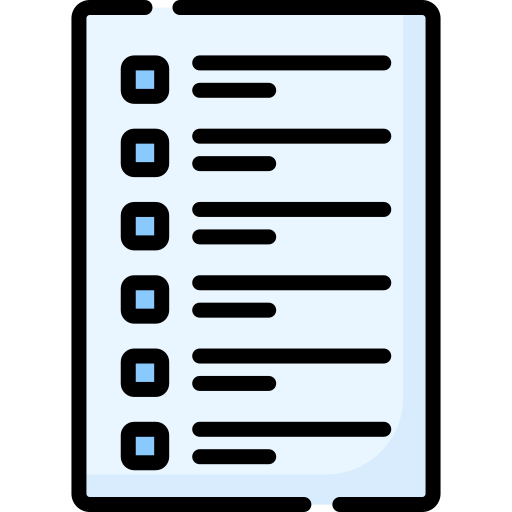
\includegraphics[width=1cm]{img/list.png}
                    & 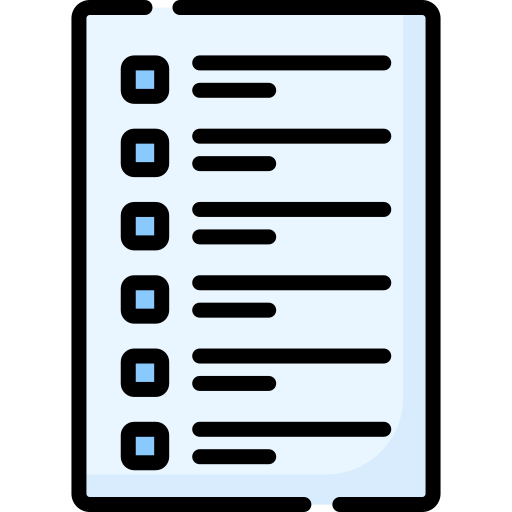
\includegraphics[width=1cm]{img/list.png}\\
    
                    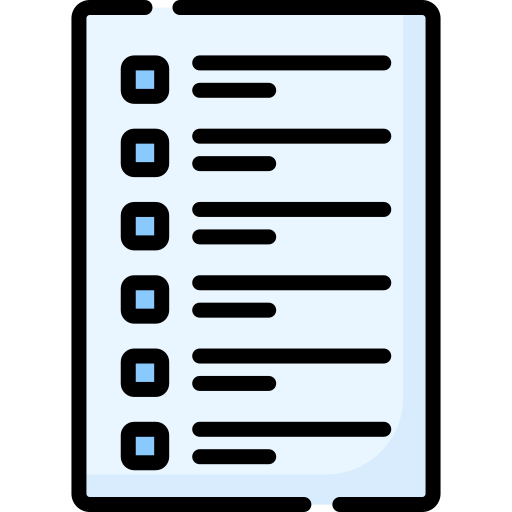
\includegraphics[width=1cm]{img/list.png}
                    & 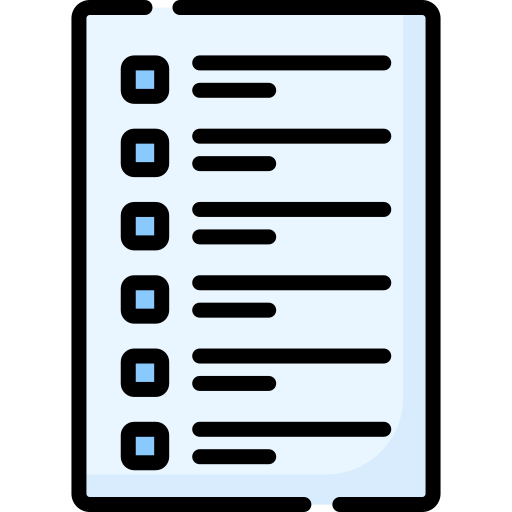
\includegraphics[width=1cm]{img/list.png}
                    & 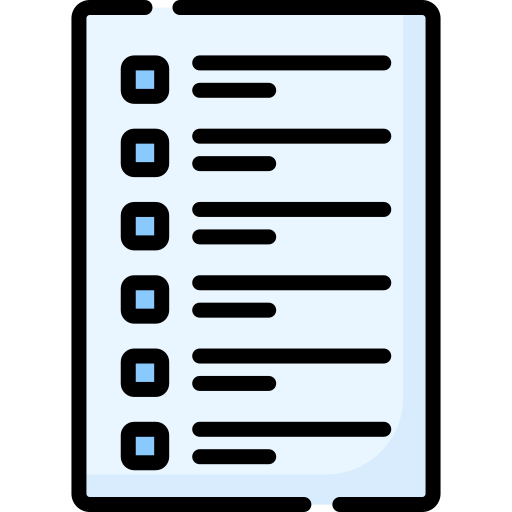
\includegraphics[width=1cm]{img/list.png}\\
    
                    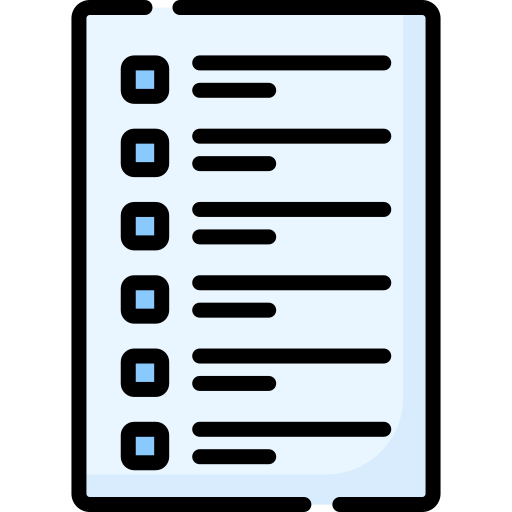
\includegraphics[width=1cm]{img/list.png}
                    & 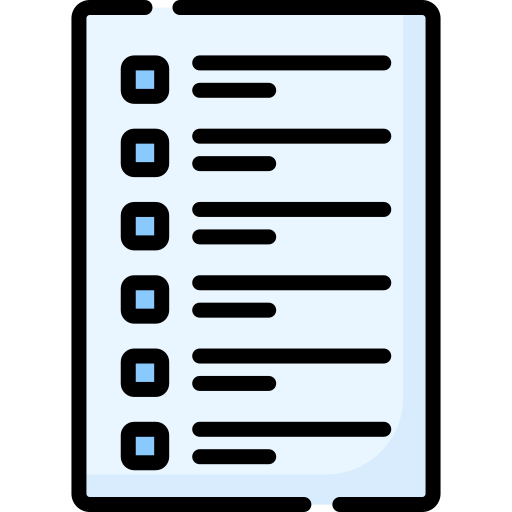
\includegraphics[width=1cm]{img/list.png}
                    & 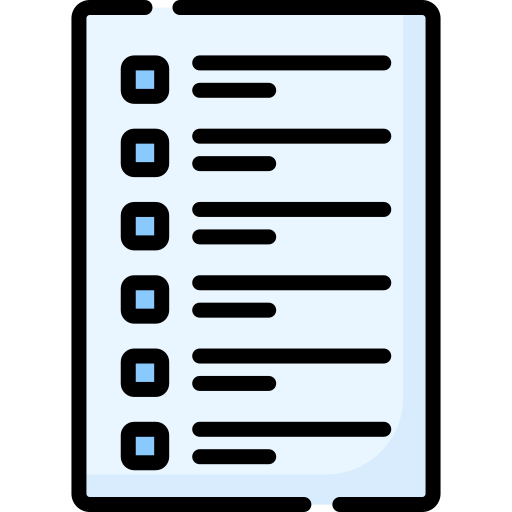
\includegraphics[width=1cm]{img/list.png}\\
    
    
                    ... & ... & ...\\
    
                    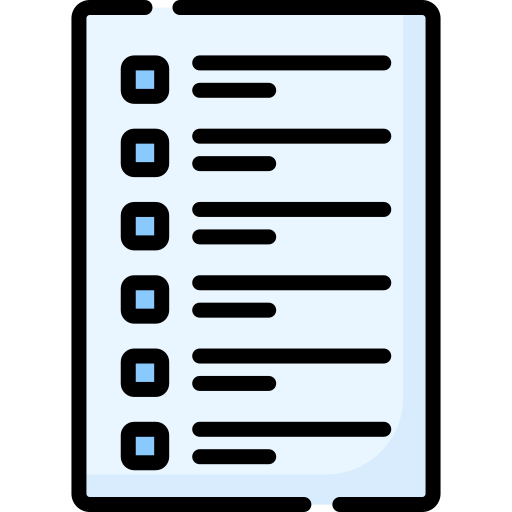
\includegraphics[width=1cm]{img/list.png}
                    & 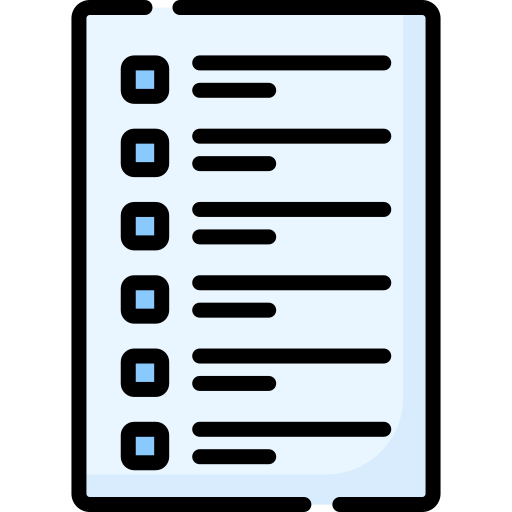
\includegraphics[width=1cm]{img/list.png}
                    & 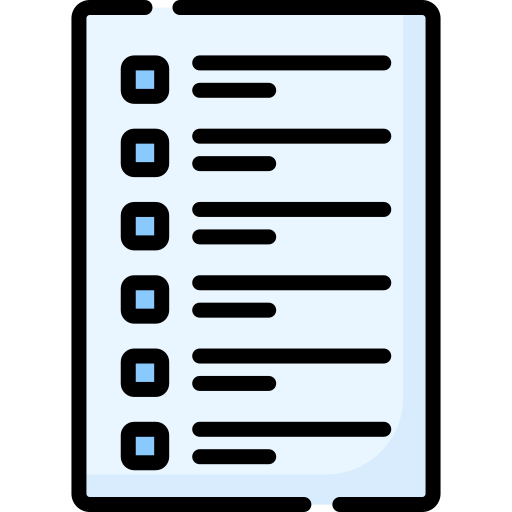
\includegraphics[width=1cm]{img/list.png}\\
    
                    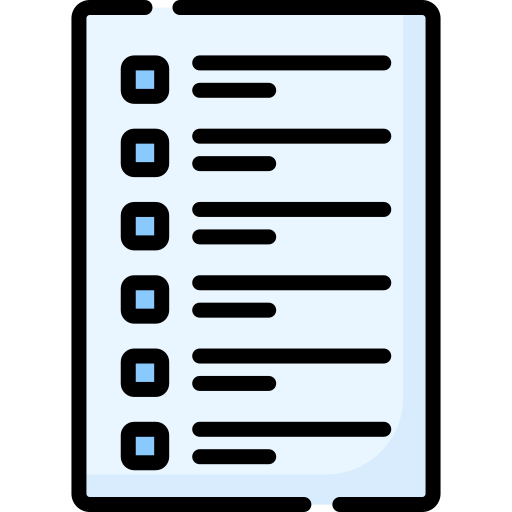
\includegraphics[width=1cm]{img/list.png}
                    & 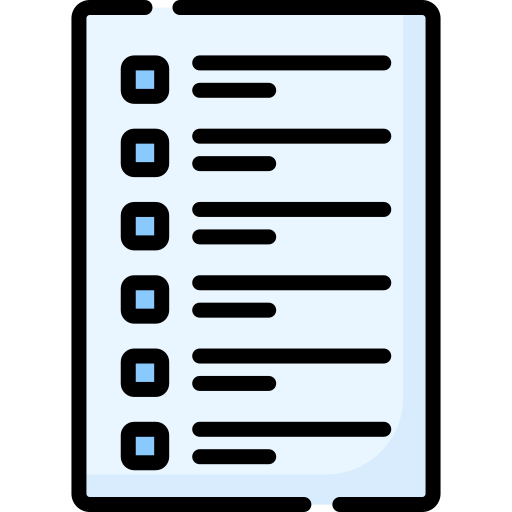
\includegraphics[width=1cm]{img/list.png}
                    & 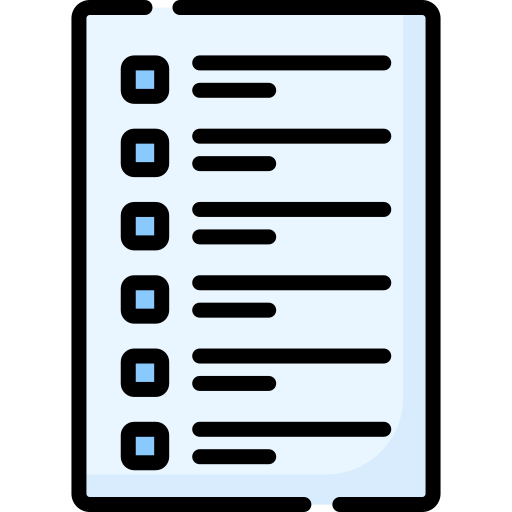
\includegraphics[width=1cm]{img/list.png}\\
    
                \end{tabular}
            \end{block}
            
    \end{column}

    


        \begin{column}{0.68\linewidth}
            \begin{block}{Caracter\'isticas}
                \begin{itemize}
                    \item Se crean nuevos ficheros a medida que se crean nuevos tipos de registros o se terminan los ficheros.
                    \item Cada fichero se opera de forma independiente del resto de archivos en almacenamiento.
                \end{itemize}
                 
            \end{block}
            \begin{alertblock}<2->{Limitaciones}
                \begin{itemize}
                    \item<2-> Baja eficiencia
                    \item<3-> Gran redundancia de los datos
                    \item<4-> Pobre control sobre los datos
                    \item<5-> Capacidades inadecuadas de manipulaci\'on de datos
                \end{itemize}
            \end{alertblock}
        \end{column}

    \end{columns}
\end{frame}